\documentclass[a4paper, conference]{IEEEtran}
\IEEEoverridecommandlockouts
% The preceding line is only needed to identify funding in the first footnote. If that is unneeded, please comment it out.
%Template version as of 6/27/2024

\usepackage[colorlinks=true, linkcolor=black, citecolor=blue, urlcolor=blue]{hyperref}

\usepackage[table]{xcolor}

\usepackage{multirow}
\usepackage{cite}
\usepackage{amsmath,amssymb,amsfonts}
\usepackage{algorithmic}
\usepackage{graphicx}
\usepackage{textcomp}
\usepackage{xcolor}
\def\BibTeX{{\rm B\kern-.05em{\sc i\kern-.025em b}\kern-.08em
	T\kern-.1667em\lower.7ex\hbox{E}\kern-.125emX}}
\begin{document}

%\title{Conference Paper Title*\\
	%{\footnotesize \textsuperscript{*}Note: Sub-titles are not captured for https://ieeexplore.ieee.org  and
		%should not be used}
	%\thanks{Identify applicable funding agency here. If none, delete this.}
	%}
%
%\author{\IEEEauthorblockN{1\textsuperscript{st} Given Name Surname}
	%\IEEEauthorblockA{\textit{dept. name of organization (of Aff.)} \\
		%\textit{name of organization (of Aff.)}\\
		%City, Country \\
		%email address or ORCID}
	%\and
	%\IEEEauthorblockN{2\textsuperscript{nd} Given Name Surname}
	%\IEEEauthorblockA{\textit{dept. name of organization (of Aff.)} \\
		%\textit{name of organization (of Aff.)}\\
		%City, Country \\
		%email address or ORCID}
	%\and
	%\IEEEauthorblockN{3\textsuperscript{rd} Given Name Surname}
	%\IEEEauthorblockA{\textit{dept. name of organization (of Aff.)} \\
		%\textit{name of organization (of Aff.)}\\
		%City, Country \\
		%email address or ORCID}
	%\and
	%\IEEEauthorblockN{4\textsuperscript{th} Given Name Surname}
	%\IEEEauthorblockA{\textit{dept. name of organization (of Aff.)} \\
		%\textit{name of organization (of Aff.)}\\
		%City, Country \\
		%email address or ORCID}
	%\and
	%\IEEEauthorblockN{5\textsuperscript{th} Given Name Surname}
	%\IEEEauthorblockA{\textit{dept. name of organization (of Aff.)} \\
		%\textit{name of organization (of Aff.)}\\
		%City, Country \\
		%email address or ORCID}
	%\and
	%\IEEEauthorblockN{6\textsuperscript{th} Given Name Surname}
	%\IEEEauthorblockA{\textit{dept. name of organization (of Aff.)} \\
		%\textit{name of organization (of Aff.)}\\
		%City, Country \\
		%email address or ORCID}
	%}

\title{\title{Towards an IT Framework for Remote Work Implementation: A Qualitative Analysis of Employee Perceptions}
}


%\author{\IEEEauthorblockN{1\textsuperscript{st} Alfa Yohannis}
%	\IEEEauthorblockA{\textit{Department of Informatics} \\
%		\textit{Universitas Pradita}\\
%		Tangerang, Indonesia \\
%		alfa.ryano@gmail.com}
%%	\and
%%	\IEEEauthorblockN{2\textsuperscript{nd} Alexander Waworuntu}
%%	\IEEEauthorblockA{\textit{Department of Informatics} \\
%%		\textit{Universitas Multimedia Nusantara}\\
%%		Tangerang, Indonesia\\
%%	alex.wawo@umn.ac.id}
%%	\and
%%	\IEEEauthorblockN{3\textsuperscript{rd} Master Edison Siregar}
%%	\IEEEauthorblockA{\textit{Department of Informatics} \\
%%		\textit{Universitas Pradita}\\
%%		Tangerang, Indonesia \\
%%		master.edison@pradita.ac.id}
%%	%\and
%%	%\IEEEauthorblockN{4\textsuperscript{th} Given Name Surname}
%%	%\IEEEauthorblockA{\textit{dept. name of organization (of Aff.)} \\
%%		%\textit{name of organization (of Aff.)}\\
%%		%City, Country \\
%%		%email address or ORCID}
%%	%\and
%%	%\IEEEauthorblockN{5\textsuperscript{th} Given Name Surname}
%%	%\IEEEauthorblockA{\textit{dept. name of organization (of Aff.)} \\
%%		%\textit{name of organization (of Aff.)}\\
%%		%City, Country \\
%%		%email address or ORCID}
%%	%\and
%%	%\IEEEauthorblockN{6\textsuperscript{th} Given Name Surname}
%%	%\IEEEauthorblockA{\textit{dept. name of organization (of Aff.)} \\
%%		%\textit{name of organization (of Aff.)}\\
%%		%City, Country \\
%%		%email address or ORCID}
%	}

 \author{\textbf{[Hidden for double-blind review]}}
%\author{\IEEEauthorblockN{
%		Alfa Yohannis%\IEEEauthorrefmark{1}
%		\IEEEauthorrefmark{2},
%		Master Edison Siregar%\IEEEauthorrefmark{1}%\IEEEauthorrefmark{3}
%	}
%	\IEEEauthorblockA{
%		% \IEEEauthorrefmark{1}
%		Hidden for Double-blind Review
%		Department of Informatics\\
%		Pradita University, Tangerang, Indonesia\\
%		\IEEEauthorrefmark{2}alfa.ryano@pradita.ac.id}
%	% 	% \IEEEauthorblockA{
%		% 	% 	\IEEEauthorrefmark{2}Department of Computer Science\\
%		% 	% 	University of York, York, United Kingdom}
%}

\newcommand{\al}[1]{{\textbf{\color{blue} Al: #1}}}

\maketitle

\begin{abstract}
	This paper presents a qualitative study on employees' perceptions of the transition from office-based work to remote work in Indonesia. The study aims to identify the perceived advantages, disadvantages, technological needs, and ethical considerations associated with remote work practices. Data were collected through an online questionnaire distributed to employees from various industries between February and May 2023. A total of 97 responses were analysed using qualitative thematic analysis to categorise the key themes emerging from the data. The findings reveal that employees recognise flexibility, time efficiency, and reduced commuting costs as key advantages of remote work, while communication barriers, work-life balance issues, and technical challenges are among the main disadvantages. Additionally, the study identifies employees' expectations regarding supporting technologies and ethical norms in remote work environments. Based on these findings, an IT framework is proposed to guide organisations in effectively implementing remote work practices. The dataset generated in this study has been made publicly available to support further research and practical applications in the Indonesian context.
\end{abstract}


\begin{IEEEkeywords}
Remote Work Implementation, Employee Perceptions, IT Framework, Digital Work Environment, Qualitative Analysis
\end{IEEEkeywords}


\section{Introduction}
The COVID-19 pandemic has fundamentally changed the way employees and organisations conduct work activities. Many companies around the world shifted from office-based work environments to remote work arrangements to ensure business continuity and employee safety. This transition has introduced both benefits and challenges, particularly in regions where remote work culture and digital infrastructure were previously underdeveloped. In Indonesia, the shift to remote work practices has revealed various factors affecting employee productivity, communication, well-being, and the ethical dimensions of remote work.

While several studies have investigated the effectiveness of remote work globally, limited research has focused on the Indonesian context, particularly from the perspective of employees across different industries. Understanding the perceived advantages, disadvantages, technological needs, and ethical considerations is crucial for organisations seeking to adopt or improve remote work policies.

This study aims to address this gap by collecting and analysing qualitative data on employees' perceptions of remote work and office-based work in Indonesia. The dataset was gathered through an online survey and includes insights into work preferences, technology use, and ethical concerns related to remote work. Based on the analysis, the study proposes a structured IT framework to support effective remote work implementation. The key contributions of this research are as follows: (1) providing a qualitative dataset on remote and office-based work perceptions in Indonesia; (2) identifying the perceived benefits and challenges of different work arrangements; (3) capturing employees' expectations regarding supporting technologies and ethics; and (4) proposing an IT framework to facilitate the implementation of remote work practices.

\section{Related Work}

Recent scholarly attention has increasingly focused on the transformation of work arrangements, particularly remote and hybrid models, following the global disruptions caused by the COVID-19 pandemic. Several studies have examined the impacts, challenges, and emerging frameworks associated with these new work patterns.

Yang et al.~\cite{yang2022effects} explored the effects of remote work on collaboration among information workers, highlighting a significant reduction in synchronous communication and cross-team collaboration. Their large-scale study demonstrated that remote work, while increasing flexibility, may inadvertently reduce the breadth of employees’ collaborative networks.

Similarly, Newbold et al.~\cite{Newbold2022NewNormals} proposed a comprehensive framework to understand organisational responses to new ways of working. Their research categorised adaptive strategies in response to remote work disruptions, offering insights into the socio-technical adjustments required at both individual and organisational levels.

In the context of digital transformation, Münch et al.~\cite{munch2022capabilities} examined digital servitization capabilities through the lens of socio-technical systems theory. Their findings emphasised the interplay between technological infrastructures and organisational processes in enabling remote service delivery.

A longitudinal perspective on the changing world of work was provided by Leonardi et al.~\cite{Leonardi2024RemoteWork}, who synthesised theoretical and empirical research to analyse how remote work reshapes organisational structures, employee autonomy, and work-life boundaries. Their work underscored the need for new managerial practices to accommodate remote work complexities.

At the firm level, Raj et al.~\cite{Raj2023Remote} conducted a global analysis to assess the relationship between remote working adoption and organisational performance. Their empirical findings indicated that remote work positively correlates with firm performance when supported by effective digital infrastructure and managerial readiness.

Building on the relational aspects of remote work, Keppler and Leonardi~\cite{Keppler2023RelationalConfidence} investigated the role of digital technologies in fostering knowledge sharing and relational confidence among remote and hybrid workers. Their study identified specific practices that can mitigate the relational distance often associated with distributed work environments.

Further addressing the implications of remote work policies, Smite et al.~\cite{Smite2023WFHFlexibility} argued for greater flexibility in post-pandemic work policies. Their research highlighted the long-term sustainability of work-from-home arrangements and the necessity of organisational policy reforms to accommodate employee preferences.

Fan and Moen~\cite{Fan2023SubjectiveWellbeing} examined the relationship between remote work modalities and subjective well-being. Their study revealed that employees working remotely or in hybrid settings reported higher levels of well-being compared to those returning to full-time office work, reinforcing the importance of flexibility and autonomy in contemporary work arrangements.

Clarifying the conceptual underpinnings of hybrid work, Lauring and Jonasson~\cite{Lauring2024Hybrid} provided a critical review of the hybrid work model. Their work addressed inconsistencies in terminology and highlighted the potential consequences of hybrid arrangements on employee engagement and organisational culture.

Finally, Choudhury et al.~\cite{Choudhury2024Hybrid} conducted a field experiment to assess the effectiveness of hybrid work models. Their findings supported the notion that hybrid arrangements can offer a balance between productivity and employee satisfaction, positioning hybrid work as a viable long-term strategy.

Collectively, these studies provide a multidimensional understanding of remote and hybrid work models, encompassing their organisational, technological, relational, and psychological dimensions. The literature reveals that while remote and hybrid work arrangements offer flexibility and potential performance benefits, they also pose challenges related to collaboration, well-being, and organisational culture that require thoughtful managerial responses.

While previous studies have provided valuable insights into the impacts, frameworks, and organisational strategies related to remote and hybrid work arrangements~\cite{yang2022effects,Newbold2022NewNormals,munch2022capabilities,Leonardi2024RemoteWork,Raj2023Remote,Keppler2023RelationalConfidence,Smite2023WFHFlexibility,Fan2023SubjectiveWellbeing,Lauring2024Hybrid,Choudhury2024Hybrid}, most of these studies were conducted in Western contexts and focused primarily on macro-level aspects such as organisational performance, collaboration patterns, or policy development. Furthermore, they often relied on experimental data, conceptual models, or large-scale quantitative analysis, overlooking the specific socio-cultural conditions of emerging economies and the detailed perceptions of individual employees. In contrast, this research addresses these gaps by collecting primary data from employees across various industries and cities in Indonesia. It adopts an inductive qualitative approach to explore employees’ perceptions regarding the advantages, disadvantages, ethical considerations, and technological aspects of remote and office-based work. The novelty of this study lies in its contextual focus on the Indonesian workforce, which is underrepresented in existing literature, and its comprehensive mapping of employee-driven insights. Additionally, this study proposes an IT framework grounded in the empirical data collected, offering practical guidance tailored to the needs and conditions of employees in Indonesia. This contribution extends the current understanding of remote work implementation by providing contextual evidence and actionable recommendations specific to developing country settings.


\section{Methodology}
\label{sec:methodology}

The data used in this research was collected through an online survey\footnote{The questionnaire is available at 
	[Hidden for double-blind review]
%	\url{https://forms.gle/phfgBDmFPEVUU95R8}
} 
conducted between February and May 2023 using the Google Forms platform. The questionnaire was designed to capture respondents' perceptions regarding the advantages, disadvantages, ethical considerations, and technological aspects of remote work and office-based work for employees in Indonesia. On the first page of the survey, it was explicitly stated that the data collected would be used solely for research purposes and handled responsibly. Participants were informed of their right to opt out at any time, and their responses would be removed accordingly.

The questionnaire was distributed to employees working in various industries through multiple online channels, including social media platforms such as Facebook, LinkedIn, and Instagram, as well as messenger applications like WhatsApp and Signal. Additionally, the survey link was shared via direct conversations and group chats to ensure broader reach and participation. The respondents were located in several cities within Indonesia, including Jakarta, Tangerang, Depok, Bogor, and Bekasi.

The data collected through the questionnaires were compiled into a comma-separated values (CSV) file. The dataset contains information in the Indonesian language, with some parts translated into English; however, the accuracy of the English content is not guaranteed. The dataset was produced specifically as part of this research to capture employees' views on remote and office-based work in Indonesia. 

This study employed a qualitative research approach. Qualitative methods are appropriate for analysing large volumes of textual data by categorising responses into thematic groups \cite{hamilton2019qualitative,kumar2018qualitative}. An inductive qualitative analysis technique was applied to identify patterns and group similar responses based on their meaning. The identified themes were then arranged according to the frequency with which they were mentioned by respondents \cite{seixas2018qualitative,turale2020brief}. This approach enabled a systematic organisation of the data, providing a clearer understanding of employees' perspectives on remote and office-based work.


The questionnaire used in this study was designed to collect information related to the respondents' demographic profile, job characteristics, and perceptions of remote work and office-based work. These variables were selected to provide a comprehensive understanding of employees' experiences and views on different work arrangements in Indonesia. The questionnaire consisted of both demographic questions and open-ended questions aimed at exploring the perceived advantages, disadvantages, ethical considerations, and technological aspects of remote and office-based work.

The variables included in the questionnaire cover key dimensions such as gender, age, industry sector, job role, job responsibilities, and perceptions of work arrangements. Specifically, the open-ended questions were structured to capture respondents' opinions on the benefits and drawbacks of working from home (WFH), working from the office (WFO), and working from anywhere (WFA), as well as the technologies they use or expect to support remote work. Additionally, the questionnaire included questions related to the mindset and ethics required in remote work settings and the perceived feasibility of remote work implementation in Indonesia. The detailed descriptions of each variable included in the dataset are summarised in Table~\ref{Data Explanation}.

\begin{table*}[ht]
	\centering
	\caption{Description of Data Fields}
	\label{Data Explanation}
	\begin{tabular}{|p{0.02\textwidth}|p{0.18\textwidth}|p{0.72\textwidth}|}
		\hline
		\textbf{No} & \textbf{Field} & \textbf{Description} \\ 
		\hline
		\textbf{1} & Gender & Information about the gender of the respondents. \\ 
		\hline
		\textbf{2} & Age & Age range of the respondents. \\ 
		\hline
		\textbf{3} & Industry & Information on the respondents' current workplace or industry. \\ 
		\hline
		\textbf{4} & Job Role & Respondents' current position or role at their respective workplaces. \\ 
		\hline
		\textbf{5} & Job Task and Responsibility & Descriptions of the respondents' daily job tasks, duties, or responsibilities related to their respective roles. \\ 
		\hline
		\textbf{6} & Advantages of WFH & Perceived benefits or positive aspects of working from home (WFH) related to the respondents' jobs. \\ 
		\hline
		\textbf{7} & Disadvantages of WFH & Perceived drawbacks or negative aspects of working from home (WFH) related to the respondents' jobs. \\ 
		\hline
		\textbf{8} & Advantages of WFO & Perceived benefits or positive aspects of working from the office (WFO) related to the respondents' jobs. \\ 
		\hline
		\textbf{9} & Disadvantages of WFO & Perceived drawbacks or negative aspects of working from the office (WFO) related to the respondents' jobs. \\ 
		\hline
		\textbf{10} & Advantages of WFA & Perceived benefits or positive aspects of implementing Work From Anywhere (WFA) related to the respondents' jobs. \\ 
		\hline
		\textbf{11} & Disadvantages of WFA & Perceived drawbacks or negative aspects of implementing Work From Anywhere (WFA) related to the respondents' jobs. \\ 
		\hline
		\textbf{12} & Technology Used in Remote Work & Technologies or applications used by the respondents during WFH or WFA to support their work. \\ 
		\hline
		\textbf{13} & Expected Technology in Remote Work & Technologies or applications that the respondents expect to support their work during remote working. \\ 
		\hline
		\textbf{14} & Mindset in Remote Work & Collection of mindsets, ethics, norms, and expected behaviours when engaging in remote work. \\ 
		\hline
		\textbf{15} & Feasibility of Remote Work in Indonesia & Respondents' perceptions of the challenges and feasibility of implementing remote work in Indonesia. \\ 
		\hline
	\end{tabular}
\end{table*}




\section{Results and Discussion}
\label{sec:results}

This section presents the results of the data collection and the discussion of the key findings. The analysis focuses on the perceptions of employees in Indonesia regarding remote work and office-based work, based on the responses gathered through the online survey. The discussion is organised to highlight the key themes identified from the qualitative analysis, supported by relevant data and interpretations.

In total, we collected responses from 97 respondents. Furthermore, the dataset has been made publicly available on Zenodo at 
[hidden for double-blind review]
%\url{https://doi.org/10.5281/zenodo.13741856} 
%\cite{yohannis2024wfo}
.

\subsection{Respondent Industry Profile}
\label{sec:respondent-industry}

The respondents in this study were drawn from various industry sectors to ensure a diverse range of perspectives regarding remote and office-based work. Table~\ref{Respondent Industry} presents the distribution of respondents based on their respective industries.

As shown in Table~\ref{Respondent Industry}, the majority of respondents work in the education sector, accounting for 29 participants. This is followed by the information technology (IT) sector with 19 respondents. Both sectors are closely associated with knowledge-based work, which typically allows greater flexibility in adopting remote work arrangements. Other sectors represented include government institutions and consulting services, each with 7 respondents, as well as clean water supply and property/real estate sectors, each with 6 respondents. Additionally, the finance sector is represented by 5 respondents, and the health sector by 3 respondents. A significant number of respondents, totalling 18, indicated that they work in industries outside the predefined categories and were classified under the \textit{Others} category.

The diversity of industries reflected in the respondent profile provides a broad perspective on the feasibility, advantages, and challenges of remote and office-based work in Indonesia. It is particularly relevant in understanding how perceptions may vary across sectors with different operational characteristics and technological readiness.


\begin{table}[ht]
	\caption{Number of Respondents per Industry}
	\label{Respondent Industry}
	\begin{tabular}{|p{.02\textwidth}|p{.35\textwidth}|r|}
		\cline{1-3}
		\textbf{No.} & \textbf{Industry}      & \textbf{Count}   \\ \hline
		\textbf{1}  & Education (Edu)     & 29            \\ \hline
		\textbf{2}  & Information Technology (IT)         & 19 \\ \hline %6 --Sebelumnya             
		\textbf{3}  & Government (Gov)     & 7             \\ \hline
		\textbf{4}  & Consulting (Cons)     & 7 \\ \hline %3 Sebelumnya
		\textbf{5}  & Clean Water Supply (CWS) & 6          \\   \hline
		%Penambahan Property, Finance, dan Health
		\textbf{6}  & Property/Real Estate (Property)     & 6             \\ \hline
		\textbf{7}  & Finance (Fin)     & 5             \\ \hline
		\textbf{8}  & Health (Health)    & 3             \\ \hline
		\textbf{9}  & Others (Other)       & 18 %46 Sebelumnya
		\\ \hline
	\end{tabular}
\end{table}

\subsection{Perceived Advantages of Working from Home}
\label{sec:advantage-wfh}

The questionnaire included an open-ended question that asked respondents to describe the perceived advantages of working from home (WFH). The qualitative responses were analysed and grouped into several themes based on the similarity of their meanings. Table~\ref{Advantage of WFH} presents the frequency of each identified theme.

As shown in Table~\ref{Advantage of WFH}, the most frequently mentioned advantage of WFH is \textit{time flexibility and time efficiency}, cited by 76 respondents. This reflects the respondents' appreciation of the ability to manage their working hours more flexibly and efficiently when working remotely. The second most common advantage is the absence of a need for commuting or travelling, mentioned by 38 respondents. This finding is consistent with previous studies that highlight the elimination of commuting time as a significant benefit of remote work.

Another advantage identified is cost-saving, particularly in relation to transportation expenses, as reported by 30 respondents. This is followed by increased productivity and the ability to perform other tasks, mentioned by 28 respondents. Additionally, 22 respondents highlighted the positive impact of WFH on their well-being, indicating improvements in comfort, reduced stress, or better work-life balance. Lastly, 17 respondents noted that WFH provided them with more time to spend with their family.

These findings indicate that the perceived advantages of WFH are largely related to flexibility, efficiency, and personal well-being, which align with the broader literature on remote work practices.

\begin{table}[ht]
	\caption{Advantage WFH}
	\label{Advantage of WFH}
	\begin{tabular}{|p{.02\textwidth}|p{.35\textwidth}|r|}
		\hline
		\multicolumn{1}{|c|}{\textbf{No.}} & \multicolumn{1}{c|}{\textbf{The Themes of WFH Advantages}} & \textbf{Count} \\ \hline
		\textbf{1}                 & Time flexibility/Time efficiency (FlexEff)         &76 %32
		\\ \hline
		\textbf{2}                 & No need for commuting/travelling (NoCom)        & 38 %9
		\\ \hline
		\textbf{3}                 & Cost-saving/Transportation expenses (Cost)        & 30 %19
		\\ \hline
		\textbf{4}                 & Increased productivity/Ability to do other tasks (Prod)& 28 %10
		\\ \hline
		\textbf{5}                 & Well-Being (Well)        & 22     
		\\ \hline
		\textbf{6}                 & More time for family (Fam)              & 17 %10
		\\ \hline
	\end{tabular}
\end{table}

\subsection{Perceived Disadvantages of Working from Home}
\label{sec:disadvantage-wfh}

In addition to identifying the advantages of working from home (WFH), the questionnaire also included an open-ended question regarding the perceived disadvantages of WFH. The responses were analysed and categorised into several thematic groups. Table~\ref{Disadvantages of WFH} summarises the identified themes along with the frequency of each theme mentioned by the respondents.

As shown in Table~\ref{Disadvantages of WFH}, the most frequently reported disadvantage of WFH is the \textit{difficulty in time management and task management}, cited by 45 respondents. This indicates that, despite the flexibility offered by WFH, many respondents experienced challenges in organising their working hours and managing their tasks effectively. The second most common disadvantage is \textit{difficulty in communication}, mentioned by 39 respondents, which reflects the limitations of remote communication tools in facilitating effective interaction and collaboration.

Furthermore, 38 respondents reported experiencing \textit{difficulty in maintaining work-life balance} while working from home. This suggests that the physical merging of home and work environments may blur boundaries and create additional stress. Another key disadvantage mentioned by 33 respondents is the \textit{difficulty in building professional relationships}, indicating the perceived negative impact of remote work on networking and social interaction in professional contexts.

Technical challenges and technology-related issues were identified by 27 respondents, highlighting concerns related to internet connectivity, hardware limitations, and software reliability. Additionally, 18 respondents mentioned a \textit{lack of motivation and self-discipline} as a challenge when working remotely, while 9 respondents reported negative impacts on their \textit{mental or physical well-being}.

These findings illustrate that, although WFH offers flexibility and convenience, it also introduces several challenges related to communication, self-regulation, social interaction, and well-being.


\begin{table}[ht]
	\caption{Disadvantages of WFH}
	\label{Disadvantages of WFH}
	\begin{tabular}{|p{.02\textwidth}|p{.35\textwidth}|r|}
		\hline
		\multicolumn{1}{|c|}{\textbf{No.}} & \multicolumn{1}{c|}{\textbf{The Themes of WFH Disadvantages}} & \multicolumn{1}{c|}{\textbf{Count}} \\ \hline
		\textbf{1}                 & Difficulty in time management and task management (Manage) & 45 %7
		\\ \hline
		\textbf{2}                 & Difficulty in Communication (Com) & 39 %7
		\\ \hline
		\textbf{3}                 & Difficulty in maintaining work-life balance (Balance)    & 38 %12
		\\ \hline
		\textbf{4}                 & Difficulty in building professional relationships (Relation)  & 33 %7
		\\ \hline
		\textbf{5}                 & Technical challenges and technology issues (Issue)     & 27
		%8
		\\ \hline
		\textbf{6}                 & Lack of motivation and self-discipline (Mov)       & 18 %9
		\\ \hline
		\textbf{7}                 & Mental or physical well-being (Well) & 9               \\ \hline
	\end{tabular}
\end{table}


\subsection{Perceived Advantages of Working from the Office}
\label{sec:advantage-wfo}

The questionnaire also explored respondents' perceptions of the advantages of working from the office (WFO). The responses were analysed and categorised into thematic groups based on the similarity of their content. Table~\ref{Advanatage of WFO} presents the identified themes along with the frequency of each theme mentioned by the respondents.

As shown in Table~\ref{Advanatage of WFO}, the most frequently mentioned advantage of WFO is \textit{effective communication and collaboration}, cited by 62 respondents. This highlights the importance of direct, face-to-face communication in facilitating clearer, faster, and more productive interactions in the workplace. The second most common advantage is the presence of \textit{strong social interaction and work relationships}, mentioned by 33 respondents. This indicates that working from the office fosters opportunities for building professional networks and maintaining social connections with colleagues.

Additionally, 42 respondents noted that WFO contributes to \textit{increased focus and productivity}. This suggests that the structured work environment of the office may help employees concentrate better and complete tasks more efficiently, without the distractions often encountered in remote settings.

These findings reflect that, while remote work offers flexibility, many employees still recognise the value of office-based work in supporting communication, collaboration, and social interaction.


\begin{table}[ht]
	\caption{Advantages of WFO}
	\label{Advanatage of WFO}
	\begin{tabular}{|p{.02\textwidth}|p{.35\textwidth}|r|}
		\hline
		\multicolumn{1}{|c|}{\textbf{No.}} & \multicolumn{1}{c|}{\textbf{The Themes of WFO advantages}} & \multicolumn{1}{c|}{\textbf{Count}} \\ \hline
		\textbf{1}             & Effective communication and collaboration (Effect)     & 62 %44
		\\ \hline
		\textbf{2}             & Strong social interaction and work relationships (Relation)& 33 %26
		\\ \hline
		\textbf{3}             & Increased focus and productivity (Prod)        & 42 %23
		\\ \hline
	\end{tabular}
\end{table}

\subsection{Perceived Disadvantages of Working from the Office}
\label{sec:disadvantage-wfo}

The questionnaire also explored the perceived disadvantages of working from the office (WFO) through an open-ended question. The responses were analysed and categorised into thematic groups based on their content. Table~\ref{Disadvantages of WFO} summarises the identified themes along with the frequency of each theme mentioned by the respondents.

As presented in Table~\ref{Disadvantages of WFO}, the most frequently mentioned disadvantage of WFO is the \textit{long and tiring commuting time}, reported by 56 respondents. This finding highlights that the time and effort required to commute to the office is considered a significant burden by many employees, which may negatively affect their well-being and productivity. The second most common disadvantage is the \textit{lack of flexibility in work hours}, mentioned by 37 respondents. This reflects employees' concerns about rigid working schedules associated with office-based work, which may limit their ability to manage personal commitments and work-life balance.

Additionally, 27 respondents noted the \textit{high transportation costs} as a disadvantage of WFO, indicating that daily commuting imposes a financial burden on employees. Lastly, 14 respondents mentioned other disadvantages that did not fall into the predefined categories. These responses include various concerns related to office-based work environments, such as workplace distractions and less autonomy.

These findings indicate that the main disadvantages of WFO are related to time, cost, and flexibility constraints, which contrast with the perceived advantages of remote work arrangements.


\begin{table}[ht]
	\caption{Disadvantages of WFO}
	\label{Disadvantages of WFO}
	\begin{tabular}{|p{.02\textwidth}|p{.35\textwidth}|r|}
		\hline
		\multicolumn{1}{|c|}{\textbf{No.}} & \multicolumn{1}{c|}{\textbf{The Themes of WFO Disadvantages}} & \multicolumn{1}{c|}{\textbf{Count}} \\ \hline
		\textbf{1}             & Long and tiring commuting time            & 56 %41
		\\ \hline
		\textbf{2}             & Lack of flexibility in work hours          & 37 %30
		\\ \hline
		\textbf{3}             & High transportation costs              & 27 %42
		\\ \hline
		\textbf{4}             & Other          & 14
		\\ \hline
	\end{tabular}
\end{table}


\subsection{Perceived Advantages of Working from Anywhere}
\label{sec:advantage-wfa}

The questionnaire also included a question to explore the respondents' perceptions of the advantages of working from anywhere (WFA). The responses were analysed qualitatively and categorised into thematic groups. Table~\ref{Advantages of WFA} presents the identified themes along with the frequency of each theme mentioned by the respondents.

As shown in Table~\ref{Advantages of WFA}, the most frequently mentioned advantage of WFA is the \textit{influence of a work environment}, cited by 61 respondents. This theme reflects the respondents' appreciation of the ability to choose or adjust their working environment based on their preferences, which may enhance comfort, motivation, and overall productivity. The second most common advantage is \textit{more flexible working hours}, mentioned by 55 respondents. This indicates that respondents value the temporal flexibility offered by WFA, allowing them to manage their work schedules according to their personal needs.

Additionally, 7 respondents identified \textit{cost savings on transportation} as a benefit of WFA, similar to one of the advantages reported for WFH. This reflects the financial benefit of not having to commute regularly when working from locations other than the office.

Overall, these findings suggest that the perceived advantages of WFA are primarily related to environmental flexibility, temporal flexibility, and reduced commuting costs, providing employees with greater autonomy in managing their work conditions.

\begin{table}
	\centering
	\caption{Advantages of WFA}
	\label{Advantages of WFA}
	\begin{tabular}{|p{.02\textwidth}|p{.35\textwidth}|r|}
		\hline
		\multicolumn{1}{|c|}{\textbf{No.}} & \multicolumn{1}{c|}{\textbf{The Themes of WFA advantages}} & \multicolumn{1}{c|}{\textbf{Count}} \\ \hline
		\textbf{1} & Influence of a work environment (Env) & 61 %72
		\\ \hline
		\textbf{2} &  More flexible working hours (Flex)       & 55 %65 
		\\ \hline
		\textbf{3} & Cost savings on transportation (Cost)      & 7 %54 
		\\ \hline
	\end{tabular}
\end{table}


\subsection{Perceived Disadvantages of Working from Anywhere}
\label{sec:disadvantage-wfa}

The questionnaire also included an open-ended question to explore respondents' perceptions of the disadvantages of working from anywhere (WFA). The qualitative responses were analysed and categorised into thematic groups based on their meaning. Table~\ref{Disadvantages of WFA} summarises the identified themes along with the frequency of each theme mentioned by the respondents.

As shown in Table~\ref{Disadvantages of WFA}, the most frequently mentioned disadvantage of WFA is \textit{difficulties in coordination and communication}, reported by 27 respondents. This theme reflects the challenges encountered in maintaining effective communication and collaboration when employees are working from different and potentially unpredictable locations. The second most common disadvantage is the \textit{limitation of infrastructure and technology}, mentioned by 26 respondents. This indicates that WFA is often constrained by factors such as internet availability, device reliability, and access to appropriate software.

Additionally, 5 respondents identified \textit{difficulties in social interaction and togetherness} as a drawback of WFA, highlighting the potential for reduced social engagement and collaboration among team members. A further 35 respondents provided responses categorised under \textit{Other}, which included various concerns such as difficulty in maintaining work discipline, distractions in the chosen work environment, or uncertainty about company policies related to remote work.

These findings suggest that, while WFA offers flexibility, it also introduces challenges related to communication, infrastructure, and social interaction, which may affect employees' productivity and well-being.


\begin{table}
	\centering
	\caption{Disadvantes of WFA}
	\label{Disadvantages of WFA}
	\begin{tabular}{|p{.02\textwidth}|p{.35\textwidth}|r|}
		\hline
		\multicolumn{1}{|c|}{\textbf{No.}} & \multicolumn{1}{c|}{\textbf{The Themes of WFA Disadvantages}} & \multicolumn{1}{c|}{\textbf{Count}} \\ \hline
		\textbf{1}                 & Difficulties in Coordination and Communication (Com)   & 27 %13
		\\ \hline
		\textbf{2}                 & Limitation of Infrastructure and Technology (Lim)    & 26 %18
		\\ \hline
		\textbf{3}                 & Difficulties in Social Interaction and Togetherness (Soc) & 5 %9
		\\ \hline
		\textbf{4}                 & Other (Other) & 35 %9
		\\ \hline
	\end{tabular}
\end{table}

\subsection{Applications Used for Remote Work}
\label{sec:used-applications}

The questionnaire also gathered information on the applications and digital platforms used by respondents to support remote work activities. This information was intended to identify the technological tools that facilitate communication, collaboration, and task management in remote work settings. The responses were categorised based on the type and function of the applications. Table~\ref{Used Application for Remote Work} presents the categories, specific products mentioned by the respondents, and the frequency of each category's mention.

As shown in Table~\ref{Used Application for Remote Work}, the most frequently mentioned category is \textit{Office Suite / Workspace}, with a total of 176 mentions. This category includes commonly used applications such as Microsoft Office 365 (including OneDrive, Excel, MS Word, PowerPoint, and SharePoint) and Google's workspace tools (such as Google Docs, Google Sheets, Google Drive, Gmail, Google Calendar, and Google Classroom). These applications are essential for document creation, file storage, and general work administration in remote settings.

The second most frequently mentioned category is \textit{Online Meeting and Video Conference Platforms}, with 148 mentions. This category includes applications such as Zoom, Microsoft Teams, Google Meet, Skype, and Webex. These platforms are fundamental for facilitating synchronous communication and virtual meetings among remote workers.

Additionally, 84 mentions were recorded under the \textit{Other Software and Platforms} category. This category covers a wide range of applications, including project management tools (Trello, Asana, Monday.com), creative software (Adobe Creative Cloud, Canva), collaboration platforms (Miro, Padlet), development tools (GitLab, GitHub, Bitbucket), and various support tools for productivity, communication, and security.

Lastly, 32 mentions were recorded under the \textit{Other Communication Applications} category. This includes messaging platforms such as WhatsApp, Telegram, Signal, LINE, and Facebook Messenger, which are widely used for informal and real-time communication among team members.

These findings illustrate the diversity of technological tools utilised by employees to facilitate remote work, reflecting the importance of digital infrastructure in supporting effective remote work practices.

\begin{table*}
	\caption{Used Application for Remote Work}
	\label{Used Application for Remote Work}
	\begin{tabular}{|p{0.24\textwidth}|p{0.64\textwidth}|r|}
		\hline
		\multicolumn{1}{|c|}{\textbf{Category}}                                            & \multicolumn{1}{c|}{\textbf{Product}}                                                 & \multicolumn{1}{c|}{\textbf{Count}} \\ \hline
		\textbf{Office Suite / Workspace (Office)} &
		OneDrive, Excel, MS Word, PowerPoint, SharePoint, Office 365, Google Docs, Google Sheets, Google Drive, Gmail, Google Calendar, Google Slides, Google Jamboard, Google Forms, Google Sites, Google Classroom & 176 %116
		%One Drive, Excel, MS Word, PowerPoint, SharePoint, Office 365, Google Docs Google Sheets, Google Drive, Gmail, etc.        & 176 %116
		\\ \hline
		\textbf{Application / Platform for Online Meeting / Video Conference (Meet)} &
		Zoom, Microsoft Teams, Google Meet, Skype, Webex, GoToMeeting, Discord, Jitsi, Around & 148 %165 % Zoom,  Microsoft Teams, Google Meet, Skype, Webex, GoToMeeting, Discord, Slack & 148 %165
		\\ \hline
		\textbf{Other Software / Platform (Other)} & Adobe Creative Cloud, Trello, Asana, Monday.com, Quizziz, Jira, Miro, Padlet, Canva, Capcut, VN editing, ClickUp, Qase, GitLab, GitHub, Bitbucket, Moodle, Prezi, Mentimeter, Kahoot, Standup.ly, SAP, TeamViewer, Anydesk, Fortinet client, Global protect, Jenkins, Greatday, HRIS, Teramind, Virtual Lab, Visual Studio, Microsoft Visio, WPS Office, PDF, Power BI, MURAL, Notion, Grammarly, QuillBot, VS Code, Figma, AWS, Adobe Sign, Vpn, STS & 84 %72   
		%Adobe Creative Cloud, Trello, Asana, Slack, Monday.com               & 84 %72              
		\\ \hline
		\textbf{Others communication Apps (Com)}                                        & WhatsApp, Telegram, Signal, LINE, Facebook Messenger, Outlook, Slack & 32 %57
		%WhatsApp, Telegram, Signal, LINE, Facebook Messenger                & 32 %57              
		\\ \hline
	\end{tabular}
\end{table*}


\subsection{Desired Applications and Technologies for Remote Work}
\label{sec:desired-apps}

The questionnaire also included an open-ended question to explore respondents' expectations regarding applications and technologies that could further support and enhance their remote work experience. The responses were categorised based on the type and purpose of the desired applications. Table~\ref{tab:required_apps_for_remote_work} presents the identified categories, examples of specific items mentioned by the respondents, and the frequency of mentions for each category.

As shown in Table~\ref{tab:required_apps_for_remote_work}, the most frequently mentioned category is \textit{Other applications and software}, with 42 mentions. This category includes various software and features requested by respondents, such as Microsoft Office, Google applications, online attendance and monitoring software, signal stabilizer software, and other digital productivity tools.

The second most mentioned category is \textit{Communication and Collaboration Applications}, with 30 mentions. Respondents highlighted the need for reliable communication platforms such as Zoom, Google Meet, Microsoft Teams, and integrated interaction tools that support effective collaboration in remote settings. Some respondents also mentioned the integration of artificial intelligence-based tools, such as ChatGPT, to improve work efficiency.

The third category is \textit{Internet and IT Infrastructure}, with 28 mentions. Respondents expressed the need for stable, high-speed, and portable internet connections that can support remote work activities without disruption.

In addition, 26 mentions were recorded for the \textit{Technology and Devices} category, which includes expectations related to the provision of laptops, high-specification devices, smartphones, tablets, and built-in internet connectivity in hardware provided by employers.

Respondents also mentioned the need for \textit{Supporting Applications for Work and Productivity}, with 19 mentions. These include systems for time management, progress monitoring, and result-based performance evaluation. Furthermore, some respondents expressed interest in advanced technologies such as \textit{Artificial Intelligence, IoT, and Machine Learning}, recorded under the \textit{AI, IoT, and Machine Learning} category, with 10 mentions.

A smaller number of respondents, 7 in total, expressed interest in immersive technologies such as \textit{VR and 3D Virtual Meeting platforms}. Lastly, 9 mentions were recorded in the \textit{Other Systems} category, which includes requests for innovative systems such as Mini World platforms, software feature upgrades, and enhanced digital learning media.

These findings indicate that employees’ expectations for supporting technologies in remote work extend beyond basic communication tools and include infrastructure, hardware, advanced technology, and integrated digital systems to improve work effectiveness and experience.

\begin{table*}
	\centering
	\caption{Desired applications to have for remote work.}
	\label{tab:required_apps_for_remote_work}
	\begin{tabular}{|p{0.25\textwidth}|p{0.63\textwidth}|r|}
		\hline
		\multicolumn{1}{|c|}{\textbf{Category}}                                   & \multicolumn{1}{c|}{\textbf{Item}}                                                                                                                                                                                   & \multicolumn{1}{c|}{\textbf{Count}} \\ \hline
		\textbf{Communication  and  collaboration apps or software (Com)} & Online Meeting Applications (Zoom, Google Meet, etc.), Interaction Integration, ChatGPT, Collaboration Applications (WhatsApp, Telegram, etc.), Microsoft Teams, Discord                                                                                     & 30 %36
		\\ \hline
		\textbf{Internet and IT infrastructure (Int)} & Stable and Fast Internet, Broadband, Portable Internet Connection, Internet that can be used anywhere, High-Speed Internet & 28 %14
		\\ \hline
		\textbf{Technology and devices (Dev)} & Laptop, High-Specification Laptops, Smartphone/Cellphone, Tablet/iPad, Signature validation, Office-provided Hardware, Built-in Internet Devices in Laptops                                                                                                                          & 26 %64
		\\ \hline
		\textbf{Supporting apps for work and productivity (Sup)} & Integrated System, Technology for Calculating Work Progress, Time Management, Kanban Board, Result-Based System & 19 %8
		\\ \hline
		\textbf{AI, IoT, and  Machine  Learning (AI)} & AI, IoT, Machine Learning
		& 10 %12
		\\ \hline
		\textbf{VR and 3D  Virtual Meeting (VR)} & VR, 3D Virtual Meeting & 7%4
		\\ \hline
		\textbf{Other applications and software (Oapp)} & Microsoft Office (Excel, Word, etc.), Google Software, Free Software, Online Attendance Software, Presentation Recording Software, Online Exam Monitoring Software, Signal Stabilizer Software, Voice-Based Report Generator Software, Integrated Company Devices, Single Sign-On, Digital Intelligence Assistance, Mobile Monitor Extender & 42 %18
		\\ \hline
		\textbf{Other system (Osys)} & Mini World, 2D to 4D Projector, Software Feature Upgrades, Integrated Administration System, Enhanced MS Teams, Digitalization of Learning Media & 9 %13
		\\ \hline
	\end{tabular}
\end{table*}

\subsection{Expected Ethics and Norms for Remote Work}
\label{sec:ethics-remote-work}

The questionnaire also included an open-ended question to identify the ethics, norms, and behavioural expectations perceived by employees as essential when engaging in remote work. The responses were analysed and categorised into four main ethical themes, each consisting of subgroups based on specific ethical aspects mentioned by the respondents. Table~\ref{tab:ethics_for_remote_work} presents the identified categories, the detailed subgroups, and the frequency of each.

As shown in Table~\ref{tab:ethics_for_remote_work}, the most frequently mentioned ethical theme is \textit{Work Ethics and Responsibilities}, with a total of 137 mentions. This category encompasses various aspects related to responsibility, discipline, and integrity in remote work. The most common subgroup under this theme is \textit{Timely Contact by Superiors, Managers, and Colleagues}, mentioned 43 times, reflecting the expectation of clear and timely communication regarding work tasks and responsibilities. Other subgroups include responsibility towards work, dress code guidelines, independence and trust, orderliness in attendance and reporting, honesty and integrity, ethical trust in the workplace, and individual responsibility in performing roles.

The second theme is \textit{Communication and Collaboration}, with 63 mentions. This category covers ethical aspects related to effective and respectful communication during remote work. The most mentioned subgroups are the expectation to \textit{Turn on the Camera during Video Calls} (21 mentions) and to practice \textit{Clear and Effective Communication} (20 mentions). Other subgroups include polite communication, proper sentence tone in emails, the need for regular meetings, and maintaining good communication practices.

The third theme is \textit{Efficiency and Productivity}, recorded with 22 mentions. This category refers to ethical practices that promote effective work processes during remote work, such as adherence to \textit{Standard Operating Procedures} (12 mentions), meeting efficiency, revision of work procedures, continuous learning, and the utilisation of screen monitoring applications.

The fourth theme is \textit{Performance Measurement}, with 20 mentions. This category reflects employees’ expectations for objective and fair performance evaluation during remote work. The majority of mentions in this category are related to \textit{Objective-Based Performance Measurement} (19 mentions), along with one mention of platform-based performance assessment.

These findings illustrate that employees expect clear ethical guidelines that cover responsibility, communication, productivity, and performance measurement to ensure professional conduct and effective collaboration in remote work environments.

\begin{table}
	\centering
	\caption{Ethics for remote work.}
	\label{tab:ethics_for_remote_work}
	\begin{tabular}{|p{0.1\textwidth}|p{0.2\textwidth}|r|r|}
		\hline
		\textbf{Ethics of Remote Work} & \textbf{Sub Group Ethics of Remote Work} & \textbf{Qty} & \textbf{Total} \\ \hline
		\multirow{8}{=}{Work Ethics and Responsibilities (Resp)}   
		& Timely Contact by Superiors with Employees, Managers, and Colleagues (Time)  & 43 & \multirow{8}{*}{137} \\ \cline{2-3}
		& Responsibility towards Work (Resp) & 30 & \\ \cline{2-3}
		& Dress Code Guidelines (Dress) & 19 & \\ \cline{2-3}
		& Independence and Trust (Ind) & 13 & \\ \cline{2-3}
		& Orderliness in Attendance Recording and Report Submission (Ord) & 13 & \\ \cline{2-3}
		& Honesty and Integrity (Hon) & 10 & \\ \cline{2-3}
		& Ethical Trust in the Workplace (Ethical) & 6 & \\ \cline{2-3}
		& Trust and Responsibility in Performing Individual Roles (Indiv) & 3 & \\ \hline
		
		\multirow{6}{=}{Communication and Collaboration (Com)}    
		& Turning on the camera during a video call (Cam) & 21 & \multirow{6}{*}{63} \\ \cline{2-3}
		& Clear and Effective Communication (Eff) & 20 & \\ \cline{2-3}
		& Polite Communication (Polite) & 13 & \\ \cline{2-3}
		& The tone of a sentence in an email (Tone) & 5 & \\ \cline{2-3}
		& Weekly Meeting to Discuss Work (Meet) & 3 & \\ \cline{2-3}
		& Good Communication (Good) & 1 & \\ \hline
		
		\multirow{5}{=}{Efficiency and Productivity (Eff)}    
		& Procedures (SOP) regarding working hours (SOP) & 12 & \multirow{5}{*}{22} \\ \cline{2-3}
		& Meeting Efficiency (Eff) & 4 & \\ \cline{2-3}
		& Revision of Standard Operating (Rev) & 3 & \\ \cline{2-3}
		& Continuous Learning (Learn) & 2 & \\ \cline{2-3}
		& Utilization of Screen Monitoring Applications (Screen) & 1 & \\ \hline
		
		\multirow{2}{=}{Performance Measurement (Perf)} 
		& Objective-Based Performance Measurement (Obj) & 19 & \multirow{2}{*}{20} \\ \cline{2-3}
		& Performance Assessment Based on Platforms (Plat) & 1 & \\ \hline
	\end{tabular}
\end{table}


\section{IT Framework Components for Remote Work Implementation}
\label{sec:it-framework}

\begin{figure*}[ht]
	\centering
	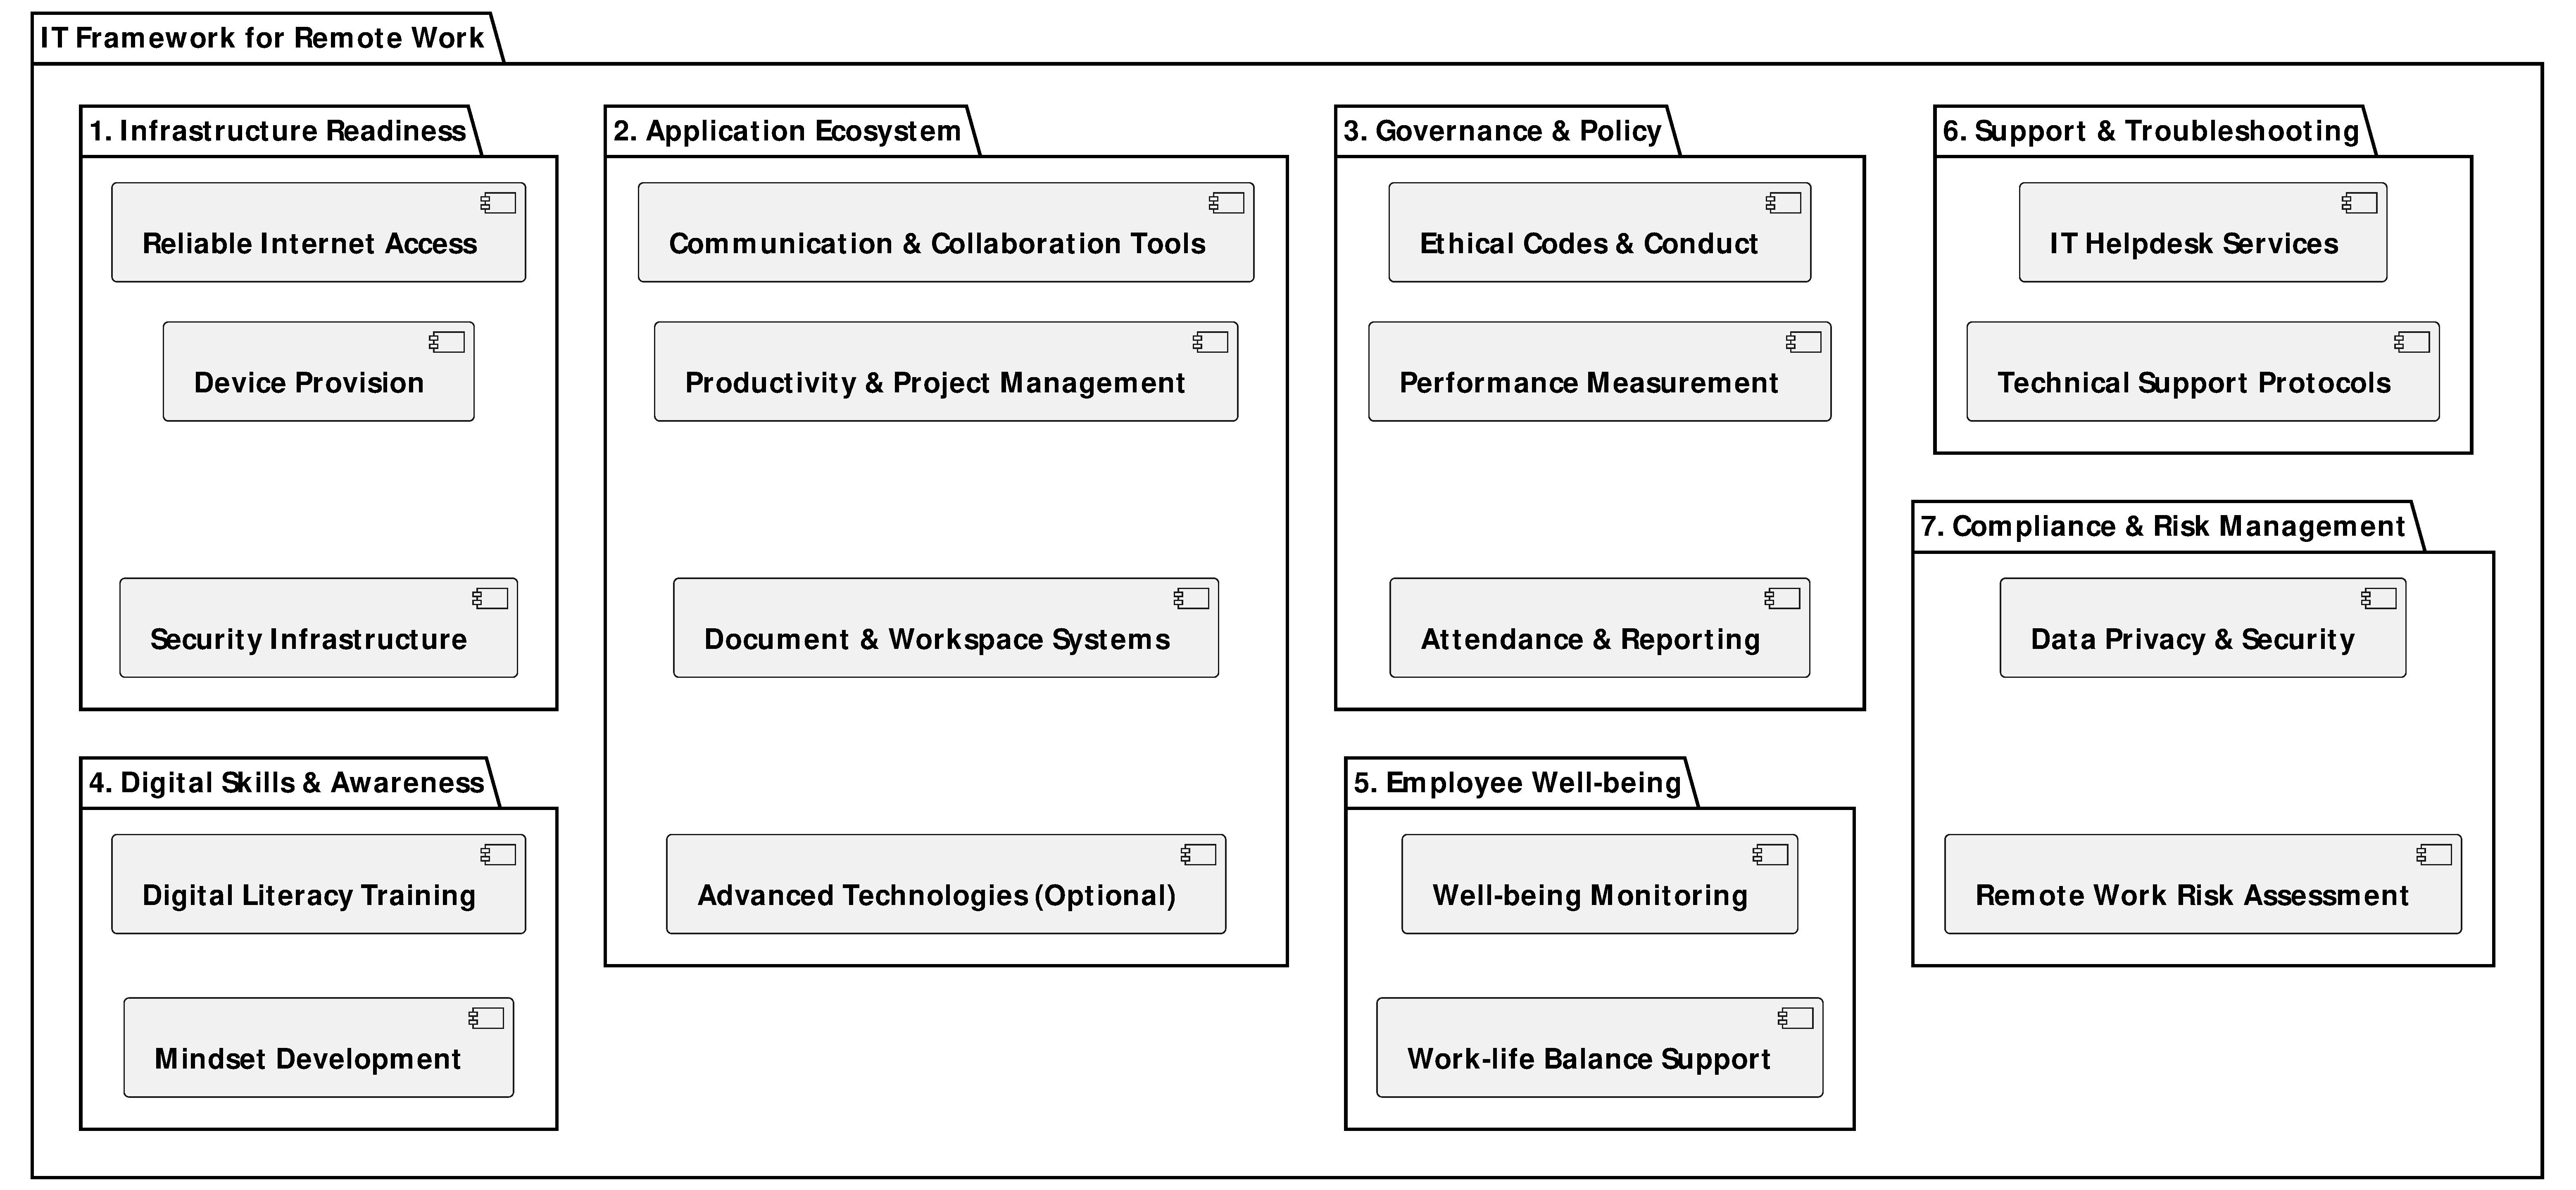
\includegraphics[width=\textwidth]{figures/out/framework.pdf}
	\caption{IT Framework Components for Remote Work Implementation}
	\label{fig:it-framework}
\end{figure*}

Based on the findings presented in Section~\ref{sec:results}, a set of essential components for an IT framework to support the implementation of remote work can be identified (Fig. \ref{fig:it-framework}). These components are derived from the analysis of respondents' perceptions regarding the advantages and disadvantages of remote work, ethical considerations, technology usage, and feasibility factors, as summarised in Tables~\ref{Advantage of WFH}, \ref{Disadvantages of WFH}, \ref{Advanatage of WFO}, \ref{Disadvantages of WFO}, \ref{Advantages of WFA}, \ref{Disadvantages of WFA}, \ref{Used Application for Remote Work}, \ref{tab:required_apps_for_remote_work}, and \ref{tab:ethics_for_remote_work}.

\textbf{Infrastructure Readiness.}
The responses indicate that reliable internet access and adequate hardware are fundamental to enabling remote work. Respondents highlighted the need for \textit{stable and high-speed internet connections} and \textit{company-provided devices} to ensure smooth remote work operations (Table~\ref{tab:required_apps_for_remote_work}). Therefore, the framework must include: (1) \textit{Reliable Internet Access} by providing internet connectivity support and ensuring employees have access to stable, high-speed internet; (2) \textit{Device Provision} by supplying standardised hardware specifications such as laptops and other supporting devices; and (3) \textit{Security Infrastructure}, which includes the implementation of VPN, single sign-on (SSO), and multi-factor authentication (MFA) systems to protect data and ensure secure access.

\textbf{Application Ecosystem.}
The findings show that employees utilise a wide range of digital applications to support remote work, including communication platforms, collaboration tools, and productivity software (Table~\ref{Used Application for Remote Work}). The framework should include an integrated ecosystem of these applications, covering: (1) \textit{Communication and Collaboration Tools}, such as Zoom, Microsoft Teams, Google Meet, and WhatsApp; (2) \textit{Productivity and Project Management Applications}, including tools for task management, progress monitoring, and collaborative work; (3) \textit{Document and Workspace Systems}, such as Office 365 and Google Workspace; and (4) \textit{Advanced Technologies (Optional)}, including AI-based assistance and virtual meeting technologies (Table~\ref{tab:required_apps_for_remote_work}).

\textbf{Governance and Policy.}
Respondents emphasised the importance of clear ethical guidelines and measurable performance indicators in remote work settings (Table~\ref{tab:ethics_for_remote_work}). To address this, the framework should include: (1) \textit{Remote Work Guidelines} covering ethical codes of conduct, dress code, communication etiquette, and working hours; (2) \textit{Performance Measurement} through objective-based evaluation systems and transparent progress reporting; and (3) \textit{Attendance and Reporting Procedures} with standardised rules for attendance recording and task reporting.

\textbf{Digital Skills and Awareness.}
The qualitative findings indicate challenges related to communication, self-discipline, and technology use (Tables~\ref{Disadvantages of WFH}, \ref{Disadvantages of WFA}). Therefore, the framework should include: (1) \textit{Capacity Building} through regular training on remote work technologies and digital literacy; and (2) \textit{Remote Work Mindset Development} programmes to foster autonomy, responsibility, and discipline.

\textbf{Employee Well-being and Work-Life Balance.}
The analysis revealed that maintaining work-life balance and well-being is a significant concern for employees (Tables~\ref{Disadvantages of WFH}, \ref{Disadvantages of WFO}). The framework should include: (1) \textit{Well-being Monitoring} channels to report stress, burnout, or other well-being issues; and (2) \textit{Work-Life Balance Policies} that encourage flexibility and set limits on working hours.

\textbf{Support and Troubleshooting Mechanism.}
Technical issues were among the challenges identified by respondents (Tables~\ref{Disadvantages of WFH}, \ref{Disadvantages of WFA}). Therefore, the framework should provide: (1) \textit{IT Helpdesk and Remote Assistance} through dedicated support channels; and (2) \textit{Technical Support Procedures} with clear protocols for addressing device, application, or connectivity issues.

\textbf{Compliance and Risk Management.}
Finally, to ensure the sustainability of remote work, the framework must incorporate compliance and risk management components, including: (1) \textit{Data Privacy and Security Compliance} to align with applicable data protection regulations; and (2) \textit{Remote Work Risk Assessment} through regular evaluation of risks related to infrastructure, ethics, and productivity.

These components form the basis of an IT framework that addresses the technical, ethical, and organisational dimensions of remote work implementation, tailored to the needs and expectations identified in the data analysis.




\section{Threats to Validity and Limitations}

This study is subject to several potential threats to validity. First, the dataset was collected through an online questionnaire using convenience sampling, which may introduce sampling bias. The participants were recruited primarily through social media and instant messaging platforms, potentially limiting the diversity and representativeness of the sample. The geographical distribution of respondents is also limited to selected cities in Indonesia, which may not reflect the experiences of employees in other regions or countries. Furthermore, the responses rely on self-reported perceptions, which may be influenced by subjective interpretations and social desirability bias.

In addition to these validity threats, this study has certain limitations. The qualitative analysis focused on thematic categorisation based on the frequency of responses, which may overlook nuanced insights or minority opinions expressed by the respondents. Moreover, the dataset was collected in early 2023, and the perceptions captured may not fully represent evolving remote work practices or policies implemented after that period. The findings and the proposed IT framework are specific to the Indonesian context and may require adjustments before being applied to other organisational or cultural settings. Future research may consider incorporating a more diverse sample and a longitudinal approach to capture changes in remote work experiences over time.


\section{Conclusion and Future Work}

This study presented a qualitative dataset and analysis of employees' perceptions regarding the transition from office-based work to remote work in Indonesia. The findings highlighted key advantages and disadvantages of remote work (WFH and WFA) and office-based work (WFO), along with employees' expectations concerning technology use and ethical considerations. Based on the analysis, an IT framework was proposed to guide organisations in implementing remote work practices, covering critical components such as infrastructure readiness, application ecosystem, governance, digital skills, employee well-being, technical support, and risk management.

Future research can expand on this work by employing a larger and more diverse sample to enhance the generalisability of the findings. Additionally, quantitative approaches or mixed-method studies can be adopted to complement the qualitative insights provided in this research. Further investigation may also focus on evaluating the effectiveness of the proposed IT framework when applied in organisational settings, as well as exploring the long-term impact of remote work practices on employee performance, well-being, and organisational productivity.


\bibliography{references}
\bibliographystyle{IEEEtran}

\end{document}
